\documentclass[11pt]{article}
\usepackage[margin=1in]{geometry}
\usepackage{times,microtype,booktabs,array,xcolor,tikz,pgfplots}
\pgfplotsset{compat=1.18}
\usetikzlibrary{arrows.meta,positioning,shapes.geometric}
\definecolor{passgreen}{RGB}{27,116,78}
\definecolor{failred}{RGB}{178,63,66}
\definecolor{warmamber}{RGB}{180,112,29}
\definecolor{deepblue}{RGB}{37,88,151}
\usepackage[hidelinks]{hyperref}
\emergencystretch=2em
\title{The Optimization That Forgot the Question:\\Verifier-Gated Code Speedups with a 1.5B Model}
\author{Tanvir Ahmed\\\small\url{https://github.com/mailtotanvir/nano-agent}}
\date{September 2026\\\textbf{Release-candidate draft --- review pending}}

\begin{document}
\maketitle
\begin{abstract}
We study whether a 1.5-billion-parameter code model can propose faster
restricted Python functions without changing what they compute. A production
controller applies one model patch and counts success only after independent
hidden-input checks and a positive Cachegrind instruction-reference reward.
A LoRA adapter trained on verifier-approved teacher traces reached 23/24 on
behavioral development (v5). Adding verified examples while removing
concentrated semantic-invariant examples coincided with a fall to 12/24
(v6); restoring focused weight recovered 21/24 (v6.1). On a frozen
seen-family split, v6.1 tied v5 at 24/30; on a frozen family-heldout split it
scored 16/30 against v5's 14/30, while both scored 0/10 on indexed lookup.
A separate three-case diagnostic yielded 0/3 for v6.1 when each candidate
omitted a required local assignment. These are one-shot, narrow-task results;
the data-mixture comparison is observational, not a causal ablation.
\end{abstract}

\section{Introduction}
An optimization is only an optimization if it preserves the question the
program answers. Counting values that appear exactly once is not the same as
counting distinct values: for $[4,4,9]$, the first answer is one and the
second is two. Both implementations may look like competent uses of a
frequency table. Similar slips arise when a rewrite removes all duplicates
instead of retaining first occurrences, or chooses the minimum rather than
the maximum sliding-window sum. These are semantic failures, not malformed
patches.

This study asks a deliberately limited question: can a small model be a
useful \emph{proposer} when an independent verifier judges both behavior and
efficiency? We report a strong development result, a marked regression after
a training-mixture change, a partial recovery, and the boundaries exposed by
frozen evaluation. The contribution is an evidence-backed account of those
boundaries, not a claim that the adapter optimizes arbitrary code.

\section{Task and verification contract}
The model receives the slow source for a pure Python function and proposes a
\textsc{search}/\textsc{replace} patch. The Rust controller applies the patch,
then delegates to a network-isolated verifier. The verifier compares the
candidate with the original on an independent edge, random, and benchmark
battery. An accepted optimization must preserve outputs on that finite
battery and improve Cachegrind instruction references under the same pinned
interpreter and verifier settings. Model-facing context excludes hidden
inputs, generator metadata, private seeds, and known-fast source. Evaluation
uses one greedy proposal per case, not a multi-attempt agent budget.

\begin{figure}[htbp]
\centering
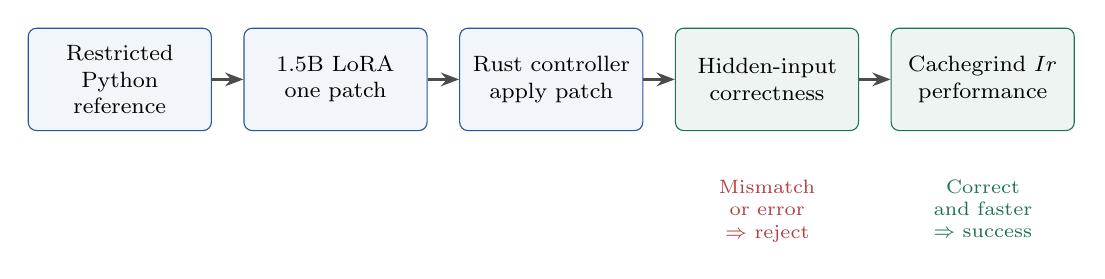
\begin{tikzpicture}[node distance=4mm,>=Stealth,
  stagebox/.style={draw=deepblue,fill=deepblue!6,rounded corners=3pt,
    align=center,text width=2.15cm,minimum height=13mm,font=\footnotesize,
    inner sep=2.5pt},
  check/.style={stagebox,draw=passgreen,fill=passgreen!8},
  arrow/.style={->,thick,draw=black!70}]
\node[stagebox] (source) {Restricted Python\\reference};
\node[stagebox,right=of source] (model) {1.5B LoRA\\one patch};
\node[stagebox,right=of model] (apply) {Rust controller\\apply patch};
\node[check,right=of apply] (correct) {Hidden-input\\correctness};
\node[check,right=of correct] (speed) {Cachegrind $Ir$\\performance};
\draw[arrow] (source)--(model);
\draw[arrow] (model)--(apply);
\draw[arrow] (apply)--(correct);
\draw[arrow] (correct)--(speed);
\node[align=center,text width=2.15cm,font=\scriptsize,text=failred,below=5mm of correct]
  {Mismatch or error\\$\Rightarrow$ reject};
\node[align=center,text width=2.15cm,font=\scriptsize,text=passgreen,below=5mm of speed]
  {Correct and faster\\$\Rightarrow$ success};
\end{tikzpicture}
\caption{The one-shot verification path. Hidden inputs, private seeds, and
known-fast source stay outside the model context. Only a correct candidate
with positive instruction-reference reward counts as success.}
\label{fig:boundary}
\end{figure}


Cachegrind's $Ir$ counts simulated instruction references for the full Python
process. It is neither wall-clock runtime nor a proof of equivalence. The
verifier is restricted to a documented subset of pure Python; it is not a
general-purpose public code-execution service. The frozen v6.1 runs used the
\texttt{code-speed-verifier:20260919} image.

\section{Experimental design}
The 24-case behavioral development split supports checkpoint comparison. The
frozen v1 benchmark has two disjoint 30-case tracks: withheld templates from
families present in training, and three entirely excluded transformation
families (string concatenation, sort selection, and indexed lookup). A new
three-case v6 residue-count-index heldout split is reported separately because
its sample is too small for a broad transfer claim. A case-ID and source audit
found no leakage from these splits into the v6.1 SFT corpus.

Every result is one greedy proposal through the same production Rust
controller and isolated verifier. A success requires both independent
hidden-input correctness and positive instruction-reference reward. The two
frozen tracks measure different transfer boundaries; their denominators are
not pooled. v5 was selected on development before v6.1 was measured on the
frozen sets. Frozen results are descriptive, not a reason to tune a further
checkpoint against those exact cases.

\section{Data and training}
The base model is \texttt{Qwen/Qwen2.5-Coder-1.5B-Instruct}. Both release
variants use PEFT LoRA rank 16, alpha 32, dropout 0.05 on attention and MLP
projection modules. Both used one epoch, learning rate $5\times10^{-5}$,
physical batch size 4, gradient accumulation 4, effective v1 replay ratio
0.4, and seed 7. A frontier teacher generated candidate trajectories;
only verifier-approved turns entered the student corpus. No new teacher
call was used for v6.1.

\begin{table}[h]
\centering\small
\begin{tabular}{lrrrp{0.34\linewidth}}
\toprule
Variant & Rows & Steps & Internal loss & Data mix \\
\midrule
v5 & 1,147 & 97 & 0.22525 & 530 verified teacher turns; 502 focused copies; 115 carryover \\
v6.1 & 1,170 & 99 & 0.18237 & 550 verified turns; 504 focused copies; one repair trace; 115 carryover \\
\bottomrule
\end{tabular}
\caption{Release variants. Internal loss is not a behavioral success metric.}
\end{table}

v6 added verified teacher examples but omitted the 502 focused copies present
in the v5 mix. Its development score fell sharply. v6.1 retained the new
verified examples and restored concentrated invariant-family weight. Its SFT
run finished 99 optimizer steps in 726.5 trainer seconds. Internal evaluation
loss was 0.1824 and assistant-token accuracy was 0.9518. Because the corpora
and training runs also differ in other respects, the v5--v6--v6.1 sequence
is not an isolated weighting ablation.

The construction sequence was explicit. First, deterministic problem rows
were verified against the restricted execution and Cachegrind harness.
Second, teacher trajectories were accepted only when the same verifier
reported correct output and positive reward. Third, training-only trajectories
were converted to assistant-only SFT targets, with grouped case-ID splitting
before replay weighting. Finally, the candidate adapter was measured on the
24-case behavioral development split. For v6.1, a prelaunch gate checked all
1,170 assistant targets (116--394 supervised tokens), leakage against the
development and frozen splits, and a one-step CPU smoke before GCP training.
The data and smoke gates establish input and training-contract integrity;
they are not behavioral success measurements.

\begin{figure}[htbp]
\centering
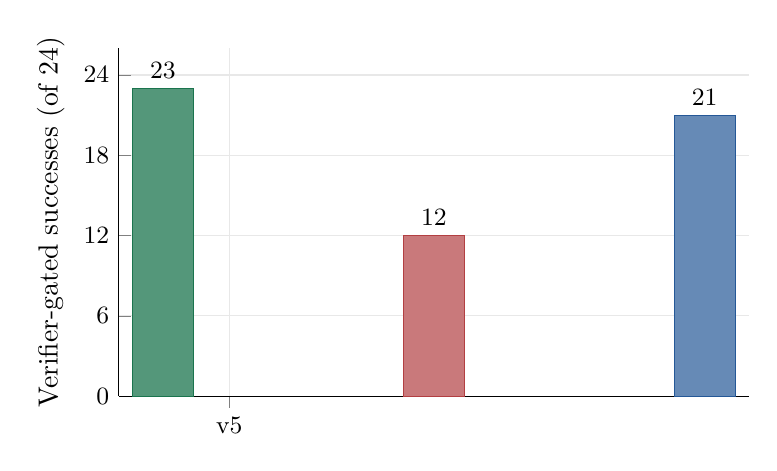
\begin{tikzpicture}
\begin{axis}[width=0.79\linewidth,height=6.0cm,ybar,bar width=22pt,
  ymin=0,ymax=26,ytick={0,6,12,18,24},ylabel={Verifier-gated successes (of 24)},
  symbolic x coords={v5,v6,v6.1},xtick=data,
  nodes near coords,every node near coord/.append style={font=\small\bfseries},
  axis x line*=bottom,axis y line*=left,grid=major,
  grid style={draw=gray!18},tick label style={font=\small},
  enlarge x limits=0.27]
\addplot[fill=passgreen!75,draw=passgreen] coordinates {(v5,23)};
\addplot[fill=failred!70,draw=failred] coordinates {(v6,12)};
\addplot[fill=deepblue!70,draw=deepblue] coordinates {(v6.1,21)};
\end{axis}
\end{tikzpicture}
\caption{Development arc on the same 24 cases, one greedy proposal each.
v5 led at 23/24; v6 fell to 12/24 when the 502 focused invariant copies were
absent; v6.1 recovered to 21/24 after focus was restored with new verified
examples retained. This is an observational data-mixture comparison.}
\label{fig:development}
\end{figure}


\section{Behavioral results}
\begin{table}[h]
\centering\small
\begin{tabular}{lcccc}
\toprule
Adapter & Dev (24) & Seen (30) & Heldout (30) & Fresh (3) \\
\midrule
v5 & 23 & 24 & 14 & Not measured \\
v6 & 12 & --- & --- & --- \\
v6.1 & 21 & 24 & 16 & 0 \\
\bottomrule
\end{tabular}
\caption{One-shot verifier-gated successes. The two frozen tracks test
different forms of generalization; the three-case diagnostic is separate.}
\end{table}

\begin{table}[htbp]
\centering\small
\begin{tabular}{lccc}
\toprule
Behavioral development family & v5 & v6 & v6.1 \\
\midrule
Hash membership & 3/3 & 3/3 & 3/3 \\
Distinct cardinality & 3/3 & 3/3 & 2/3 \\
Stable deduplication & 3/3 & 2/3 & 2/3 \\
Frequency index & 3/3 & 2/3 & 3/3 \\
Complement lookup & 3/3 & 0/3 & 3/3 \\
Running aggregate & 3/3 & 0/3 & 3/3 \\
Prefix range query & 3/3 & 2/3 & 3/3 \\
Fixed sliding window & 2/3 & 0/3 & 2/3 \\
\midrule
Total & 23/24 & 12/24 & 21/24 \\
\bottomrule
\end{tabular}
\caption{Development breakdown. v6's large losses in complement lookup and
running aggregate recover in v6.1; distinct cardinality and stable
deduplication do not fully match v5.}
\label{tab:devfamilies}
\end{table}

\begin{figure}[htbp]
\centering
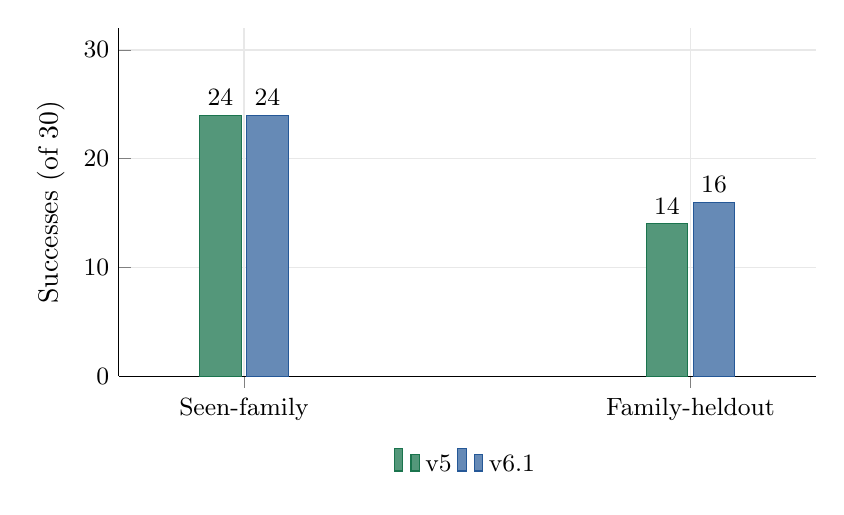
\begin{tikzpicture}
\begin{axis}[width=0.86\linewidth,height=6.0cm,ybar,bar width=15pt,
  ymin=0,ymax=32,ytick={0,10,20,30},ylabel={Successes (of 30)},
  symbolic x coords={Seen-family,Family-heldout},xtick=data,
  xticklabel style={font=\small},tick label style={font=\small},
  nodes near coords,every node near coord/.append style={font=\small},
  axis x line*=bottom,axis y line*=left,grid=major,grid style={draw=gray!18},
  enlarge x limits=0.28,legend style={at={(0.5,-0.19)},anchor=north,draw=none,
  legend columns=2,font=\small}]
\addplot[fill=passgreen!75,draw=passgreen] coordinates
  {(Seen-family,24) (Family-heldout,14)};
\addplot[fill=deepblue!70,draw=deepblue] coordinates
  {(Seen-family,24) (Family-heldout,16)};
\legend{v5,v6.1}
\end{axis}
\end{tikzpicture}
\caption{The two 30-case frozen tracks are separate questions. The seen-family
totals tie; v6.1 gains two family-heldout cases. v5 was selected on development
before v6.1's frozen measurement. These are descriptive counts, not a pooled
60-case optimization score.}
\label{fig:frozen}
\end{figure}


v5 was selected by its higher development score before v6.1 frozen
measurement. v6.1's six seen-family misses comprised five semantic failures
and one correct-but-not-faster patch. Its development misses included counting
singleton rather than distinct values, filtering duplicates rather than
keeping first occurrences, and choosing the minimum instead of maximum
fixed-window sum. The verifier rejected all three.

The equal seen-family total masks a case-level trade: v6.1 gained one case
each in complement lookup and fixed-window sums, and lost one each in
distinct cardinality and stable deduplication. Frequency index, hash
membership, prefix range query, and running aggregate totals were unchanged.

\begin{table}[htbp]
\centering\small
\begin{tabular}{lcc}
\toprule
Frozen seen-family group & v5 & v6.1 \\
\midrule
Complement lookup & 1/4 & 2/4 \\
Distinct cardinality & 3/4 & 2/4 \\
Fixed sliding window & 1/3 & 2/3 \\
Frequency index & 4/4 & 4/4 \\
Hash membership & 4/4 & 4/4 \\
Prefix range query & 3/3 & 3/3 \\
Running aggregate & 4/4 & 4/4 \\
Stable deduplication & 4/4 & 3/4 \\
\midrule
Total & 24/30 & 24/30 \\
\bottomrule
\end{tabular}
\caption{Equal seen-family totals mask two gains and two losses.}
\label{tab:seenfamilies}
\end{table}

\begin{table}[h]
\centering\small
\begin{tabular}{lcc}
\toprule
Frozen family-heldout group & v5 & v6.1 \\
\midrule
String concatenation & 7/10 & 8/10 \\
Sort selection & 7/10 & 8/10 \\
Indexed lookup & 0/10 & 0/10 \\
\bottomrule
\end{tabular}
\caption{Heldout-family results. The aggregate two-case gain is confined
to the first two groups.}
\end{table}

\begin{figure}[htbp]
\centering
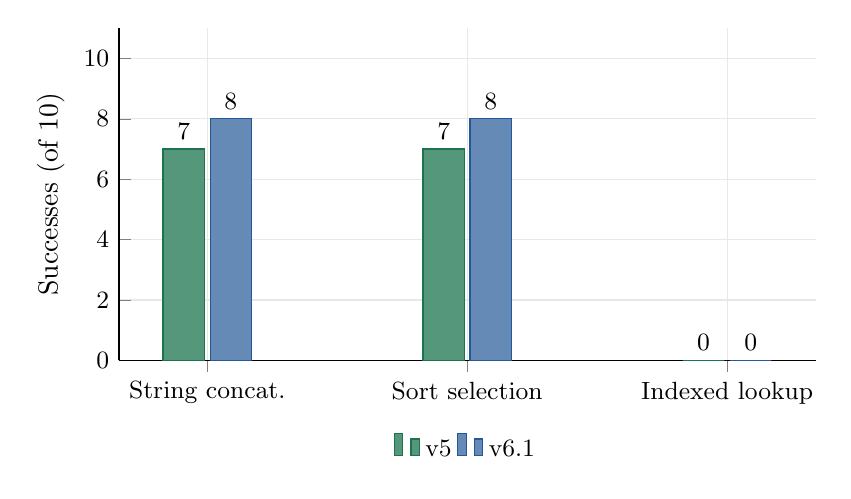
\begin{tikzpicture}
\begin{axis}[width=0.86\linewidth,height=5.8cm,ybar,bar width=15pt,
  ymin=0,ymax=11,ytick={0,2,4,6,8,10},ylabel={Successes (of 10)},
  symbolic x coords={String,Sort,Indexed},xtick=data,
  xticklabels={String concat.,Sort selection,Indexed lookup},
  tick label style={font=\small},nodes near coords,
  every node near coord/.append style={font=\small},
  axis x line*=bottom,axis y line*=left,grid=major,
  grid style={draw=gray!18},enlarge x limits=0.17,
  legend style={at={(0.5,-0.2)},anchor=north,draw=none,
  legend columns=2,font=\small}]
\addplot[fill=passgreen!75,draw=passgreen] coordinates
  {(String,7) (Sort,7) (Indexed,0)};
\addplot[fill=deepblue!70,draw=deepblue] coordinates
  {(String,8) (Sort,8) (Indexed,0)};
\legend{v5,v6.1}
\end{axis}
\end{tikzpicture}
\caption{Family-heldout decomposition. v6.1 gains one string-concatenation
and one sort-selection case; both adapters remain 0/10 on indexed lookup.
Each bar is a count over ten cases, not a population estimate.}
\label{fig:heldoutfamilies}
\end{figure}


Thirteen of v6.1's fourteen family-heldout misses were semantic failures;
one was correct but not faster. On the fresh v6 residue-count-index
diagnostic, all three v6.1 candidates omitted an in-function
\texttt{bucket\_size} assignment and therefore raised a candidate error;
one also reversed query order. v5 was not evaluated on this split. The
repeated missing dependency is a diagnostic clue, not a stable transfer rate.

\begin{figure}[htbp]
\centering
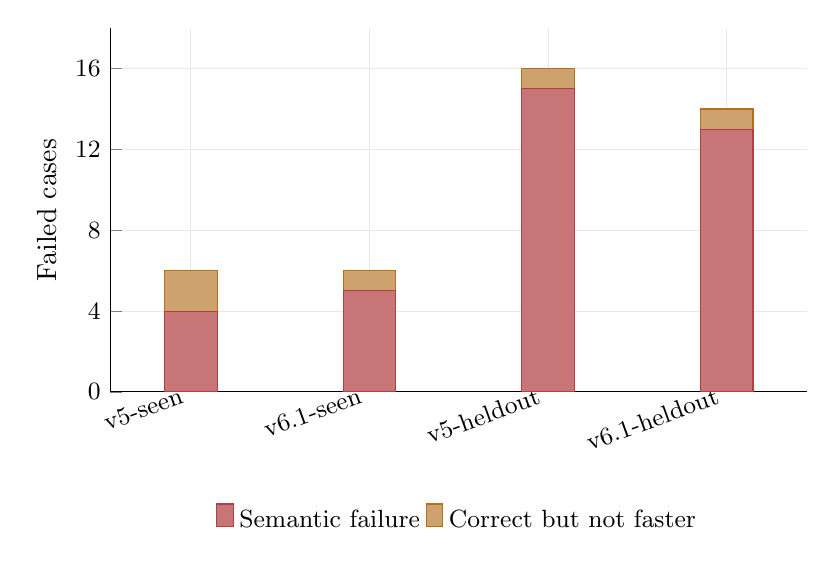
\begin{tikzpicture}
\begin{axis}[width=0.86\linewidth,height=6.2cm,ybar stacked,bar width=19pt,
  ymin=0,ymax=18,ytick={0,4,8,12,16},ylabel={Failed cases},
  symbolic x coords={v5-seen,v6.1-seen,v5-heldout,v6.1-heldout},xtick=data,
  xticklabel style={rotate=20,anchor=east,font=\small},
  tick label style={font=\small},axis x line*=bottom,axis y line*=left,
  grid=major,grid style={draw=gray!18},enlarge x limits=0.15,
  legend style={at={(0.5,-0.29)},anchor=north,draw=none,legend columns=2,
  font=\small}]
\addplot[fill=failred!72,draw=failred] coordinates
  {(v5-seen,4) (v6.1-seen,5) (v5-heldout,15) (v6.1-heldout,13)};
\addplot[fill=warmamber!65,draw=warmamber] coordinates
  {(v5-seen,2) (v6.1-seen,1) (v5-heldout,1) (v6.1-heldout,1)};
\legend{Semantic failure,Correct but not faster}
\end{axis}
\end{tikzpicture}
\caption{Failure taxonomy on frozen tracks. Semantic failures include wrong
outputs and candidate errors; ``correct but not faster'' denotes no positive
Cachegrind reward. The 0/3 fresh diagnostic is excluded because it is a
different, exploratory split.}
\label{fig:failures}
\end{figure}


\section{Interpretation and next experiment}
An independent verifier exposes fluent but behavior-changing patches and
supplies the criterion for counting success. The mixture observations
suggest that verified examples should be examined for \emph{which invariants
they reinforce}, not only counted. They do not show that focused copies alone
caused the regression and recovery; a controlled multi-seed ablation would
be needed. In particular, internal training-token fit did not predict the
development collapse or make v6.1 better than v5 on development.

The heldout result is bounded as well. v6.1's two-case advantage arose in
string concatenation and sort selection. Neither released variant solved any
indexed-lookup case, and v6.1 failed all three fresh local-dependency cases.
A next study should train on genuinely new examples that require carrying
local assignments through a rewrite, with a new heldout boundary established
before training. Reusing the current frozen cases for model selection would
undermine their independence. Multiple seeds, paired case-level analysis,
and a separately measured runtime study would strengthen future claims.

\section{Limitations and release evidence}
The model is a patch proposer for a restricted pure-Python grammar, not a
general code optimizer. Hidden tests are finite. The development set was
used for iterative choices, and repeated research can influence later
decisions even when frozen sources are withheld. Each configuration has one
training seed. One case changes a 30-case score by 3.3 percentage points;
the three-case diagnostic is too small to estimate a population rate.
Cachegrind improvement cannot be converted to wall-clock speedup.

The repository contains the controller, verifier, data pipeline, leakage
audit, SFT and evaluation code. Corpus, adapter, and report SHA-256 values
are recorded in the release manifest and model card. GCP training archives
were copied and hash-verified before the VMs and boot disks were deleted.
The recorded on-demand L4 quote was \$0.856856553/hour, under a \$1.75
two-hour authorization ceiling; actual billing is pending. Private test
inputs are not released. Base-model license and teacher-provider terms
require publisher review before a public upload. The teacher model identity
is not specified in this report, so exact teacher-data regeneration is not
claimed.

The intended model repository presents v5 and v6.1 as equal experiment
variants, without a default adapter. Equal visibility is not a claim of
equal performance. No Zenodo DOI or Hugging Face destination is asserted
before a public upload is verified.

\section*{Artifact statement}
The proposed release separates LoRA adapters into \texttt{v5/} and
\texttt{v6p1/}. The model card will link this paper, source repository, and
split-by-split evidence. A claim--evidence matrix and SHA-256 manifest
accompany the release draft. The Zenodo paper record is intended to contain
only the final PDF under a new DOI. TeX and figure source, evidence manifests,
and implementation code belong in the separate public source repository, not
in the Zenodo file list.
The companion artifacts are the \href{https://github.com/mailtotanvir/nano-agent}{source repository},
\href{https://huggingface.co/mailtotanvir/nano-agent-code-speed-1.5b}{two adapter variants},
and the \href{https://mailtotanvir.github.io/nano-agent/code-speedup-blog.html}{technical story}.

\section*{Evidence index}
All empirical claims are traceable to repository paths; private JSON reports
are retained locally with hashes rather than embedded in the paper.
\begin{enumerate}
\small\raggedright
\item \path{recipes/code-speedup/experiments/V5_BEHAVIORAL_EVALUATION_2026-09-21.md}:
  v5 development and both frozen tracks; frozen report hashes.
\item \path{recipes/code-speedup/experiments/V6_BEHAVIORAL_EVALUATION_2026-09-23.md}:
  v6 regression and semantic-failure taxonomy.
\item \path{recipes/code-speedup/experiments/V6P1_BEHAVIORAL_EVALUATION_2026-09-23.md}:
  v6.1 development by family and representative semantic failures.
\item \path{recipes/code-speedup/experiments/V6P1_FROZEN_EVALUATION_2026-09-23.md}:
  frozen family totals, per-family comparisons, fresh diagnostic, input/report
  SHA-256 values, and evaluator teardown.
\item \path{recipes/code-speedup/publication/CLAIM_EVIDENCE_MATRIX.md}:
  publication-claim boundaries and intentionally excluded claims.
\item \path{recipes/code-speedup/publication/ADAPTER_RELEASE_MANIFEST.md}:
  adapter and tokenizer SHA-256 values.
\end{enumerate}

\begin{thebibliography}{9}
\bibitem{qwen}
Qwen Team, \emph{Qwen2.5-Coder-1.5B-Instruct}, model card,
\url{https://huggingface.co/Qwen/Qwen2.5-Coder-1.5B-Instruct}.
\bibitem{peft}
Hugging Face, \emph{PEFT: Parameter-Efficient Fine-Tuning},
\url{https://github.com/huggingface/peft}.
\bibitem{cachegrind}
Valgrind Developers, \emph{Cachegrind: a cache and branch-prediction profiler},
\url{https://valgrind.org/docs/manual/cg-manual.html}.
\end{thebibliography}
\end{document}
